% =====================================================================
% SECTION 3: Dynamics  +  SECTION 4: Recurrence and the block
% =====================================================================

\section{Dynamics: The Interaction Sector on the Prime Lattice}\label{sec:dynamics}

\subsection{The frozen Hamiltonian}

The dynamical claims of the framework---transitions into composite integer states, and
factorization of the evolving state into highly composite integers---require a Hamiltonian
with off-diagonal matrix elements in the occupation basis. The primon Hamiltonian has none:

\begin{proposition}[Frozen spectrum]\label{prop:frozen}
$[H_{P},\Nhat]=0$ and $[H_{P},\hat n_{p}]=0$ for every $p$. Consequently every basis vector
$\ket{n}$ is a stationary state: $e^{-i\tau H_{P}/\hbar}\ket{n}=e^{-i\omega_{0}\tau\log
n}\ket{n}$ never leaves the ray $\Cc\ket{n}$. In particular the vacuum $\ket{1}$ is an
eigenstate with eigenvalue $0$ and evolves trivially, $e^{-i\tau H_{P}/\hbar}\ket{1}=\ket{1}$
for all $\tau$.
\end{proposition}

\begin{proof}
Both operators are diagonal in the same basis (Theorem~\ref{thm:spectrum}).
\end{proof}

A diagonal Hamiltonian cannot create primons, destroy them, or entangle anything. The
``arithmetic cascade,'' the entanglement growth, and the emergence of a thermodynamic arrow
all require dynamics \emph{off} the diagonal of $\Nhat$. The interaction sector must be
supplied. Meeting this requirement produces, as a byproduct, the objects on which the rest
of the framework rests: the multiplicative shift operators, the prime lattice, and a
well-posed thermalization problem.

\subsection{Multiplicative shift operators}

\begin{definition}[Multiplication operator]\label{def:multiplication}
For $n\in\Nn_{\geq1}$ define $M_{n}\colon\Hil_{\mathcal{A}}\to\Hil_{\mathcal{A}}$ on basis
vectors by
\begin{equation}
M_{n}\ket{k}=\ket{nk},
\end{equation}
extended linearly, with adjoint $M_{n}^{\dagger}\ket{k}=\ket{k/n}$ if $n\mid k$ (i.e.
$k_{p}\geq a_{p}$ for all $p$ with $n=\prod p^{a_{p}}$) and $M_{n}^{\dagger}\ket{k}=0$
otherwise.
\end{definition}

\begin{proposition}[Monoid representation]\label{prop:monoidrep}
The assignment $n\mapsto M_{n}$ is an isometric representation of the multiplicative monoid
$(\Nn_{\geq1},\times)$ on $\Hil_{\mathcal{A}}$:
\begin{enumerate}[leftmargin=1.6em]
\item $M_{m}M_{n}=M_{mn}=M_{n}M_{m}$ (the representation is abelian);
\item $M_{n}^{\dagger}M_{n}=I$ (each $M_{n}$ is an isometry);
\item $M_{n}M_{n}^{\dagger}=I-P(\,n\mid k\,)$, where $P(\,n\mid k\,)$ is the projection onto
$\overline{\mathrm{span}}\{\ket{k}: n\mid k\}$, a product over the modes $p^{a_{p}}\| n$ of
the projections onto $\{\hat n_{p}\geq a_{p}\}$;
\item $\|M_{n}\|=\|M_{n}^{\dagger}\|=1$, and $M_{1}=I$.
\end{enumerate}
Moreover, for each prime $p$,
\begin{equation}\label{eq:shiftladder}
M_{p}=a_{p}^{\dagger}\,(\hat n_{p}+1)^{-1/2},
\end{equation}
so $M_{p}$ is the \emph{unilateral shift} of the $p$-mode tensored with the identity on all
other modes.
\end{proposition}

\begin{proof}
(1) $M_{m}M_{n}\ket{k}=\ket{mnk}$ by associativity and commutativity of multiplication in
$\Nn$. (2) $M_{n}$ maps the orthonormal basis $\{\ket{k}\}$ to the orthonormal family
$\{\ket{nk}\}$ (distinct $k$ give distinct $nk$ by cancellation in $\Nn$), hence is an
isometry. (3) The initial space of $M_{n}^{\dagger}$ is the range of $M_{n}$, i.e. the closed
span of $\ket{k}$ with $n\mid k$; this condition factorizes across modes because divisibility
does. (4) is immediate. For \eqref{eq:shiftladder}: on $\ket{k}$,
$a_{p}^{\dagger}(\hat n_{p}+1)^{-1/2}\ket{k}=\sqrt{k_{p}+1}\,(k_{p}+1)^{-1/2}\ket{k+e_{p}}
=\ket{k+e_{p}}=M_{p}\ket{k}$.
\end{proof}

The operators $M_{n}$ are the arithmetic analogues of the Weyl shifts, and
Proposition~\ref{prop:monoidrep} is the exact statement behind the phrase that
composites are ``correlated multi-prime states'': multiplication \emph{creates} occupation,
division \emph{annihilates} it, and the two are adjoints. Note also the co-isometric defect
$M_{n}M_{n}^{\dagger}=I-P(n\mid k)$: multiplication by $n$ is invertible precisely on states
already divisible by $n$. The failure of unitarity of each individual $M_{n}$ is the
operator-theoretic fingerprint of the irreversibility that arithmetic carries:
the semigroup $(\Nn,\times)$ is
free, hence has cancellation but no inverses, and the quantum representation inherits exactly
that structure.

\subsection{The walk Hamiltonian and the prime lattice}\label{sec:walk}

Define, for a finite set $P_{f}\subset\Pr$ of active modes and real couplings
$g=(g_{p})_{p\in P_{f}}$, the \emph{multiplicative walk Hamiltonian}
\begin{equation}\label{eq:walkH}
H_{W}(P_{f},g)\;=\;\sum_{p\in P_{f}}g_{p}\bigl(M_{p}+M_{p}^{\dagger}\bigr),
\end{equation}
and the \emph{hopping Hamiltonian}
\begin{equation}\label{eq:hopH}
H_{\mathrm{hop}}(P_{f},h)\;=\;\sum_{p\neq q\in P_{f}}h_{pq}
\bigl(a_{p}^{\dagger}a_{q}+a_{q}^{\dagger}a_{p}\bigr).
\end{equation}

\begin{proposition}[Well-posed interacting dynamics]\label{prop:wellposed}
For finite $P_{f}$, $H_{W}$ and $H_{\mathrm{hop}}$ are bounded and self-adjoint. The full
Hamiltonian
\begin{equation}\label{eq:fullH}
H_{\mathrm{tot}}=H_{P}+H_{W}+H_{\mathrm{hop}}
\end{equation}
is self-adjoint on the domain of $H_{P}$ (Kato--Rellich), and
$[H_{\mathrm{tot}},\Nhat]\neq0$: the dynamics generates genuine transitions
\begin{equation}
\bra{m}H_{W}\ket{k}\neq 0 \iff m/k\in\{p,p^{-1}\}\ \text{for some }p\in P_{f},
\end{equation}
i.e. precisely the edges of the \emph{divisibility graph} of $\Nn$ restricted to $P_{f}$.
\end{proposition}

\begin{proof}
Each $M_{p}$ is bounded with norm $1$ (Proposition~\ref{prop:monoidrep}); a finite sum of
bounded self-adjoint operators is bounded self-adjoint. $a_{p}^{\dagger}a_{q}$ is bounded
(particle-number preserving hop). $H_{\mathrm{tot}}$ is a bounded perturbation of the
self-adjoint $H_{P}$, hence self-adjoint on $D(H_{P})$. Non-commutation:
$M_{p}$ changes the eigenvalue of $\Nhat$ from $n$ to $np$, and a direct computation gives
\begin{equation}
[H_{W},\Nhat]\ket{n}=\sum_{p}g_{p}\,n\Bigl(-(p-1)\ket{np}+\bigl(1-\tfrac{1}{p}\bigr)\,\mathbf{1}_{p\mid n}\ket{n/p}\Bigr)\neq0
\end{equation}
for $n\geq1$ and nonzero $g$: the two coefficients are different in both sign and magnitude
($-(p-1)$ versus $1-1/p$), so the terms cannot cancel.
\end{proof}

Three remarks interpret these objects.

\begin{remark}[The prime lattice]
$H_{\mathrm{hop}}$ is a Bose--Hubbard-type tight-binding Hamiltonian on a lattice whose
\emph{sites} are the primes, with on-site energies $\varepsilon_{p}=\hbar\omega_{0}\log p$ and
hopping $h_{pq}$. We call this graph the \emph{prime lattice}. It is the natural home for
every interaction claim in the framework: interactions among prime modes are hops along the
lattice; the chaotic sector conjectured in Conjecture~$\mathsf{C5}$ is a spectral-statistics
statement about $H_{\mathrm{tot}}$ on the prime lattice; and the ``chemistry of the
primes'' becomes the statement that the Standard Model's force sectors correspond
to structured sub-lattices (Conjecture~$\mathsf{C9}$).
\end{remark}

\begin{remark}[Conservation structure]\label{rem:conservation}
The three sectors carry a strict conservation hierarchy. $H_{P}$ is diagonal in the occupation
basis and conserves everything. $H_{\mathrm{hop}}$ moves single primons between modes
($a_{p}^{\dagger}a_{q}$: one occupation up, one down), so it conserves the \emph{total primon
number} $\Nhat_{\mathrm{tot}}=\sum_{p}\hat n_{p}$ exactly, but not $\Nhat$ (it rescales $n$ by
$q/p$). $H_{W}$ conserves \emph{neither}: each $M_{p}$ raises the occupation of the $p$-mode by
one and hence raises $\Nhat_{\mathrm{tot}}$ by one, while each $M_{p}^{\dagger}$ lowers it---the
walk is the nucleation sector, the engine of entropy growth in the precise quantitative sense
of Proposition~\ref{prop:nucleation} ($d\langle\Nhat_{\mathrm{tot}}\rangle/d\tau>0$ from
$\ket{1}$ whenever $H_{W}\neq0$). The full theory therefore has a graded conservation
hierarchy: $H_{P}$ conserves $\Nhat$ and $\Nhat_{\mathrm{tot}}$; $H_{\mathrm{hop}}$ conserves
$\Nhat_{\mathrm{tot}}$ only; $H_{W}$ conserves neither and is the only source of net primon
creation. The additive and multiplicative structures of $\Nn$ thereby acquire distinct
dynamical roles---spectral order ($H_{P}$), transport ($H_{\mathrm{hop}}$), creation
($H_{W}$)---which separates ``spectral order'' from
``arithmetic cascade.'' Register note: the CP ratchet of $\mathsf{C10}$ lives entirely in this
non-conserving $H_{W}$ sector.
\end{remark}

\begin{remark}[Relation to the reported physics]
The conformal primon gas reported near black-hole singularities~\cite{hartnollyang2026}
corresponds in this language to the claim that \emph{some} sector of
near-singularity gravity is governed by $H_{P}$ (or its Gaussian analogue) with the conformal
$\mathfrak{sl}(2,\Rr)$ symmetry of the axioms acting on the $\omega_{0}$ scale.
The interacting extension \eqref{eq:fullH} is the framework's addition; its necessity
follows from the arrow-of-time claims, which (by
Proposition~\ref{prop:frozen}) are impossible under $H_{P}$ alone.
\end{remark}

\subsection{The cascade: statics and dynamics}

The ``thermodynamic cascade'' is the framework's central image from sparse prime
states into dense composite states. As dynamics under $H_{P}$ this is impossible
(Proposition~\ref{prop:frozen}); as a statement about the \emph{microcanonical ensemble},
however, it is a classical theorem. The dichotomy therefore splits the cascade into a theorem
(statics) and a conjecture (dynamics).

\begin{theorem}[Normal order and Erd\H{o}s--Kac for the primon ensemble]\label{thm:erdoskac}
Fix $E>0$ and let $x=e^{E/\hbar\omega_{0}}$. Equip
$\{n\leq x\}$ with the uniform measure, i.e. the microcanonical ensemble of $H_{P}$ at energy
$E$. Let $\omega(n)$ be the number of distinct prime factors of $n$. Then:
\begin{enumerate}[leftmargin=1.6em]
\item (Hardy--Ramanujan \cite{hardyramanujan1917}; Tur{\'a}n \cite{turan1934}.)
$\omega(n)$ has normal order $\log\log n$: for every $\varepsilon>0$ the proportion of
$n\leq x$ with $|\omega(n)-\log\log x|>\varepsilon\log\log x$ tends to $0$ as $x\to\infty$.
\item (Erd\H{o}s--Kac \cite{erdoskac1940}.) The distribution of
$(\omega(n)-\log\log x)/\sqrt{\log\log x}$ converges to the standard Gaussian: for all $t$,
\begin{equation}
\lim_{x\to\infty}\frac{1}{x}\#\Bigl\{n\leq x:
\frac{\omega(n)-\log\log x}{\sqrt{\log\log x}}\leq t\Bigr\}=\Phi(t).
\end{equation}
\end{enumerate}
\end{theorem}

The interpretation is exact. The number of states at energy $E$ is $\lfloor e^{E/\hbar\omega_{0}}\rfloor$
(Section~\ref{sec:thermo}), and Theorem~\ref{thm:erdoskac} describes the \emph{typical} member
of that ensemble: a composite integer with about $\log\log x$ distinct prime factors,
$\log\log x=\log(E/\hbar\omega_{0})$ growing only logarithmically in the energy. The entropy
$\log N(E)=E/\hbar\omega_{0}+O(1)$ is astronomically larger than the typical complexity
$\log\log N(E)$: the ensemble is dominated by integers that are composite but \emph{far from
maximally} composite (the maximally composite integers, the powers of two and their smooth
kin, are exponentially atypical). Thus a ``cascade into composite states'' is
correct as a description of where the measure lives, and the Erd\H{o}s--Kac Gaussian is the
precise fluctuation law of the cascade. What remains open is the dynamical version:

\begin{conjecture}[Cascade/thermalization on the prime lattice, interacting completion]\label{conj:cascade}
Let
\begin{equation}\label{eq:completions}
H_{\mathrm{tot}}^{(U,V)}=H_{P}+H_{W}+H_{\mathrm{hop}}
+U\!\sum_{p<q}\hat n_{p}\hat n_{q}
+V\!\sum_{p<q}(\hat n_{p}+\hat n_{q})\bigl(a_{p}^{\dagger}a_{q}+a_{q}^{\dagger}a_{p}\bigr)
\end{equation}
on $\Hil_{\mathcal{A}}$ with generic couplings and $U\neq0$ or $V\neq0$ (diagonal or kinetic
interacting completion; both are quartic in the ladder operators, and the kinetic one is
off-diagonal and $\Nhat_{\mathrm{tot}}$-preserving, with matrix elements
$V(k_{p}+k_{q})\sqrt{(k_{p}+1)\,k_{q}}$ on the hops of the prime lattice), restricted to the
energy window $[E,E+\Delta]$. Then along any truncation
sequence with truncation dimension $D\to\infty$ at fixed effective dose: (i) eigenstate expectation values of local
occupation observables are smooth in $E$ with within-window fluctuations
$\sigma_{\mathrm{ETH}}(D)\to0$; (ii) diagonal-ensemble values converge to the microcanonical
values of Theorem~\ref{thm:erdoskac}; and (iii) the relaxation time scale is polynomial in
$E$. The bare $H_{\mathrm{tot}}$ ($U=V=0$) is \emph{excluded}: it is a quasi-quadratic object
(see below) to which the thermalization question does not apply.
\end{conjecture}

Conjecture~\ref{conj:cascade} (register entry $\mathsf{C4}$) is the engine for every
arrow-of-time claim in the framework: entropy growth, decoherence, record formation, and the
emergence of the second law are all downstream of it. It is a well-posed, hard, and
conventional-sounding problem of quantum statistical mechanics, which is exactly the point:
the framework's most sweeping physical claims reduce to questions that experts know how to
test. The two completions in \eqref{eq:completions} are not equivalent and the
difference matters: the $U$ term is a diagonal potential on the exponent lattice (a
Wannier--Stark-type renderer, as the data confirm), while the $V$ term is the
Bose--Hubbard-type \emph{density-assisted hopping} known from the interacting-boson
literature---quartic yet kinetic. Before the numerical record, the conjecture's premise
requires one piece of mathematics: the kinetic term is quartic in the occupations, hence
unbounded, so the infinite-volume operator must be shown to exist before thermalization
along truncation sequences can even be posed.

\begin{proposition}[Infinite-volume self-adjointness of the completions]\label{prop:infinitevolume}
Fix $d\geq1$ primes, real couplings, and let $H^{(K)}$ denote the box truncation of
$H_{\mathrm{tot}}^{(U,V)}$ to occupations $k_{i}\leq K$ on $\ell^{2}(\Nn^{d})$. Then:
(i) each $H^{(K)}$ is finite-dimensional and symmetric; (ii) $H_{\mathrm{tot}}^{(U,V)}$,
defined on the finite-support core $C_{0}(\Nn^{d})$, is essentially self-adjoint, with closure
self-adjoint and bounded below on the domain
$D(\Lambda)=D(H_{P})\cap D(\Nhat_{\mathrm{tot}}^{2})$ of the confining diagonal
$\Lambda=H_{P}+\lambda\Nhat_{\mathrm{tot}}^{2}$ for any
$\lambda>2\,(C_{U}+C_{V}V\,d^{2})$; and (iii) $H^{(K)}\to H_{\mathrm{tot}}^{(U,V)}$ in the
strong resolvent sense---indeed $H^{(K)}\psi=H\psi$ exactly once
$K\geq1+\max\mathrm{supp}(\psi)$, so each fixed-occupation sector of the truncation ladder
stabilizes and the thermodynamic limit is implemented without edge corrections.
\end{proposition}

\begin{proof}
Every term of $H_{\mathrm{tot}}^{(U,V)}$ changes each occupation by at most one, so
$H^{(K)}\psi=H\psi$ on core vectors of support $\leq K-1$; this gives (iii) once (ii) is in
hand, since $C_{0}$ is a core and the truncations converge on it. For (ii), write
$M=\Nhat_{\mathrm{tot}}$ and note first that $H_{\mathrm{kin}}$ and the $U$ term commute with
$M$, so both decompose along the $M$-sectors, which are finite
($\dim=\binom{M+d-1}{d-1}$). On a sector, $|U\sum_{p<q}k_{p}k_{q}|\leq U\tbinom{d}{2}M^{2}/2$,
and the kinetic term is a direct sum of finite Jacobi blocks in the coordinate of the hopping
pair (each hop moves one primon from $q$ to $p$, conserving $k_{p}+k_{q}$), with weights
$V(k_{p}+k_{q})\sqrt{(k_{p}+1)k_{q}}\leq V\,M(M+2)/2$; hence
$\|H_{\mathrm{kin}}\psi\|\leq C_{V}V d^{2}\|M^{2}\psi\|$ and
$\|H_{U}\psi\|\leq C_{U}\|M^{2}\psi\|$. For the remaining sectors,
$\|H_{\mathrm{hop}}\psi\|\leq C_{h}d^{2}\|(M+1)\psi\|$ (each amplitude
$h_{pq}\sqrt{(k_{p}+1)k_{q}}$ is linear in the occupations) and
$\|H_{W}\psi\|^{2}\leq C_{g}d\,\langle\psi,(M+1)\psi\rangle$ (each $M_{p}$ is a partial
isometry with $\|M_{p}\psi\|^{2}=\langle\psi,(\hat n_{p}+1)\psi\rangle$). Since
$x\mapsto x$ and $x\mapsto x^{1/2}$ are dominated by $x\mapsto\varepsilon x^{2}+c_{\varepsilon}$
with arbitrarily small $\varepsilon$, the last two terms are $\Lambda$-bounded with relative
bound zero, where $\Lambda\geq\lambda M^{2}$ gives
$\|\Lambda\psi\|\geq\lambda\|M^{2}\psi\|$; the first two terms therefore carry relative
bounds $(C_{U}+C_{V}Vd^{2})/\lambda$. Choosing
$\lambda>2(C_{U}+C_{V}Vd^{2})$ makes the total relative bound $<1$, and Kato--Rellich
applied to $H_{\mathrm{tot}}=\Lambda+(H_{\mathrm{tot}}-\Lambda)$ on $D(\Lambda)$ gives a
self-adjoint, bounded-below closure; essential self-adjointness on $C_{0}$ follows because
$C_{0}$ is a core of the diagonal $\Lambda$ and the bounds extend.
\end{proof}

\begin{remark}[The $d\to\infty$ limit is open]
The constants above grow with the pair count $d^{2}$: Proposition~\ref{prop:infinitevolume}
covers the thermodynamic ($K\to\infty$) limit at fixed prime number $d$. The $d\to\infty$
extension with unweighted couplings is not controlled by this argument; summable coupling
families ($\sum_{p}|g_{p}|$, $\sum_{p\neq q}|h_{pq}|$, $\sum_{p<q}|V_{pq}|$ finite) would make
the quadratic forms converge on the finite-occupation core, but we do not pursue this and
flag it as the open side of the well-posedness program.
\end{remark}

The two completions are distinguished by computation:

\begin{remark}[Numerical status of the cascade conjecture]\label{rem:numerics}
Conjecture~\ref{conj:cascade} has been tested by dense diagonalization at $D\leq4096$; by
shift-invert Lanczos eigen-windows ($k=350$ interior eigenpairs placed at the median of the
density of states, diagonal pivoting in the factorization, every window certified by
eigenpair residuals $\leq6\times10^{-8}$) up to $D=59319$ in $d=3$ and $D=20736$ in $d=4$,
beyond which the $LU$ fill exceeds the $3.4$\,GB address-space guard; by
restarted-Lanczos Krylov equilibration to $D\approx10^{5}$, with restart steps sized by a
Lanczos-estimated spectral radius (validated against exact eigendecomposition propagation
to $10^{-12}$, state-vector norm drift $\leq10^{-13}$); and by a Krylov-tier fluctuation
window past the $LU$ ceiling: plain restarted Lanczos on $H$ itself (which='LM') returns the
$k=350$ \emph{upper-edge} eigenpairs at every scale, certified to residuals
$\leq1.3\times10^{-11}$, and these feed the same window diagnostics as the shift-invert tier
($40$\,s at $D=20736$, $233$\,s at $D=104976$). The median-window Krylov routes were
measured and closed: folded-operator restarted Lanczos ($-\,(H-\sigma)^{2}$, which='LA')
stalls at subspace budgets $240$/$460$/$700$ ($0$ of $160$ wanted pairs after $60$--$121$
restart cycles---the window boundary is a spectral continuum, so no factorization-free
transform separates the $160$th from the $161$st level); LOBPCG preconditioned by a doubled
incomplete $LU$ of the shifted system is numerically unstable (indefinite double solves
overflow); unpreconditioned LOBPCG contracts at $\approx0.96$ per iteration; and a soft
Gaussian-filter estimator requires polynomial degree $\sim\|H\|/\sigma_{\mathrm{filter}}\approx5\times10^{3}$ on this band. The kinetic family is examined at
matched effective dose $VK^{2}\approx36$, the occupation-weighted coupling, so that the dose
is fixed while the truncation widens; code and data accompany the paper. The evidence:
(a) \emph{Level statistics}: generic couplings give GOE ratio statistics
$\langle r\rangle=0.45$--$0.58$ at every scale computed from $D=625$ to
$5.9\times10^{4}$ (the upper end of the band is the $d=4$, $K=11$, $D=20736$ window; the
sub-GOE values sit at the smallest matched-dose grids, $K\leq14$, where the fixed effective
dose leaves spectral mixing incomplete); the weak-coupling control collapses the
participation ratio to
$\mathrm{PR}/D\approx10^{-4}$ with $\sigma_{\mathrm{ETH}}$ inflated by an order of
magnitude, and its $\langle r\rangle$ is \emph{window-placement-dependent in a way the
generic regime is not}: a $\sigma$-quantile sweep of the same weak configuration
($d=3$, $K=28$, $D=24389$) at quantiles $\{0.02,0.10,0.15,0.25,0.5,0.75,0.9,0.98\}$
gives $0.42$--$0.56$, non-monotone (the dip at the $15\%$ quantile, $0.436$, is reproduced
exactly in an independent repetition---density-of-states cluster structure, not solver
noise),
while the generic control is flat ($0.505$--$0.514$ at quantiles $0.05/0.5/0.95$); the
weak median value is additionally direction-dependent ($0.53$ at $d=3$ versus $0.44$ at
$d=4$, $D=20736$). Any protocol claim about weak-coupling statistics must therefore pin
the quantile and the direction; the robust weak-coupling diagnostic is $\mathrm{PR}/D$,
not $\langle r\rangle$. (b) \emph{ETH fails for the bare $H_{\mathrm{tot}}$
structurally}: $H_{P}$ is a separable ramp, $H_{W}$ is a per-axis adjacency
(Wannier--Stark chains; propagation along the $p$-axis is Stark-suppressed when
$g_{p}\lesssim\log p$), and $H_{\mathrm{hop}}$ is quadratic---no quartic term exists
anywhere in $H_{\mathrm{tot}}$, so the system is essentially single-particle on the
exponent lattice $\Zz^{d}$. The scaled data make this quantitative: the normalized
eigenstate fluctuation $\sigma_{\mathrm{ETH}}/\mathrm{std}(a_{j})$ of local
occupations sits at $0.94$--$0.99$---fluctuations as large as the observable's full
spread---flat in $D$ at every coupling and every fixed dose (item (e) below); and the
time-averaged occupation retains
$6$--$24\%$ of the initial mode's occupation
($|\mathrm{diag}-\mathrm{micro}|/K$) at every scale from $D=10^{4}$ to $10^{5}$,
with no downward trend. (c) \emph{The diagonal quartic completion does not rescue
thermalization at any accessible scale}: the dose--response is monotone
localization ($\langle r\rangle$: $0.514$ at $U=0$, $0.502$ at $U=0.5$, $0.387$ at
$U=2$, all at $D\approx2\times10^{4}$; $\mathrm{PR}/D$: $0.18\to0.03\to0.001$;
frozen-mode memory $|\mathrm{diag}-\mathrm{micro}|/K\approx0.8$). (d) \emph{The kinetic (density-assisted hopping) completion}---a one-term addition to
the Hamiltonian, Hermitian and exactly $\Nhat_{\mathrm{tot}}$-preserving, validated against a
first-principles dense assembly to $10^{-15}$---is the only completion that relaxes. At
matched dose $VK^{2}\approx36$ on the $d=4$, $K=11$, $D=20736$ platform, the occupation
$\hat n_{d}$ falls from its initial value $11$ to $\approx3.5$ within $\tau\approx20$ and then
drifts on a slow secular tail; the eigenstates stay delocalized with GOE statistics
($\mathrm{PR}/D=0.14$, $\langle r\rangle=0.51$) where the quartic completion collapses to
$0.001$--$0.03$. The equilibration is a dose phenomenon, not a monotone onset: at $V=0.1$
the plateau sits \emph{away} from microcanonical ($|\mathrm{diag}-\mathrm{micro}|/K=0.18$,
the bare value; the short-horizon averages at the same platform are $0.10$ bare and $0.81$
quartic), and strong dose localizes, as the occupation-weighted matrix elements predict
(effective coupling $VK^{2}$: at $V=1$, $\langle r\rangle\to0.41$ and
$\mathrm{PR}/D\to0.05$; at fixed $V=0.3$ on the $d=3$, $K=28$ grid, where
$VK^{2}\approx235$, $\langle r\rangle=0.36$ with $\mathrm{PR}/D=0.016$).
(e) \emph{Scaling at matched dose; the diagonal ensemble.} Two legs decide the conjecture.
The eigenstate fluctuation ratio $\sigma_{\mathrm{ETH}}/\mathrm{std}(a_{j})$ is flat:
$0.95$--$0.98$ along the $d=3$ ladder $D=3375\to59319$ (a factor $17.6$ in $D$) and
$0.95$--$0.97$ along the $d=4$ median-window ladder $D=4096\to20736$, with exact full-spectrum values
$0.68$--$0.83$ at $D\leq10^{4}$; the Krylov-tier upper-edge window extends the $d=4$
measurement to $D=104976$ ($K=15$: $0.895$; $K=17$: $0.888$, against $0.871$--$0.886$ at
$K=7$--$11$---flat across a factor $25.6$ in $D$), and the $d=3$ edge ladder
($D=3375\to59319$) is flat at $0.835$--$0.839$. The bin-width control (eleven to one
hundred sixteen levels per bin) moves the ratio by less than $0.05$ at every grid where it
is computable, so the flatness is not a binning artifact. The edge windows carry their own
sector physics: $\langle r\rangle_{\mathrm{edge}}=0.38$--$0.43$ (Poisson-like, versus $0.51$
GOE at the median) and $\mathrm{PR}/D=0.054\to0.009$ (semi-localized), so the edge ladder is
reported as a second fluctuation measurement, not a substitute for the median window.
Leg (i) has no positive evidence at accessible scales. The
diagonal ensemble
$\langle a\rangle_{\mathrm{diag}}=\sum_{n}|\braket{n}{\psi_{0}}|^{2}\braket{n}{a}$
is computed exactly at $D\leq10^{4}$: there the finite-time plateau equals it to
$|\,\mathrm{plateau}-\mathrm{diag}\,|/K\leq0.005$ (the dephasing identity
$\lim_{T\to\infty}\frac{1}{T}\int_{0}^{T}\langle a(t)\rangle\,dt=\langle
a\rangle_{\mathrm{diag}}$ holds with no ETH input, and nested late-time window averages
supply the convergence diagnostic). But at matched dose the diagonal ensemble is not
microcanonical: $|\langle a\rangle_{\mathrm{diag}}-\langle
a\rangle_{\mathrm{micro}}|/K=0.040\to0.061\to0.092$ along $d=4$ ($D=4096\to20736$) and
$\approx0.05$ (stable in absolute value, $\approx0.87$) along $d=3$ ($D=3375\to9261$),
with no closing trend. The $d=4$, $D=20736$ trajectory was extended to $\tau=300$ in
checkpointed wall-clock chunks (a chunk boundary is an ordinary Lanczos restart; the resumed
trajectory agrees with an independent step-size choice to $2\times10^{-4}$ in the
observable): its nested late-time averages saturate at
$\langle\hat n_{d}\rangle_{\mathrm{diag}}\approx4.40\pm0.03$, while the microcanonical value
is $3.35$ and the early transient ($\tau\leq22$) passes through $3.39$, close to it. A
finite-horizon coincidence with the microcanonical value is therefore not evidence of
thermalization; leg (ii) is a statement about the $D\to\infty$ limit of the diagonal
ensemble, and at accessible scales that limit shows no convergence (Figure~\ref{fig:ladder}).
The matched-dose trajectories at the largest grids confirm the horizon structure: at
$D=38416$ the running average climbs through the microcanonical value on the same slow
secular tail ($3.96$ at $\tau=20$, $4.21$ at $\tau=39$, $4.43$ at $\tau=59$, microcanonical
$3.96$), and at $D=65536$ and $D=104976$ the resumable trajectories reach only
$\tau\lesssim50$ per day-scale compute, the dephasing horizon shrinking as the level spacing
does.
(The kinetic couplings destroy the diagonal dominance on which default partial pivoting
relies in the shift-invert factorization; diagonal pivoting
($\mathrm{diag\_pivot\_thresh}=0$) restores tractability---the generic $d=3$, $K=28$
factorization drops from $257$\,s to $3$\,s---with every eigen-window certified by
eigenpair residuals $\leq6\times10^{-8}$ and a pivoting cross-check at $D=14641$ agreeing
to $0.002$ in $\langle r\rangle$.) An $E\to\infty$ statement cannot be falsified by any
finite-$D$ simulation; a \emph{scaling} criterion can be---and on the present evidence
every scaling diagnostic is flat.
\end{remark}

\begin{figure}[t]
\centering
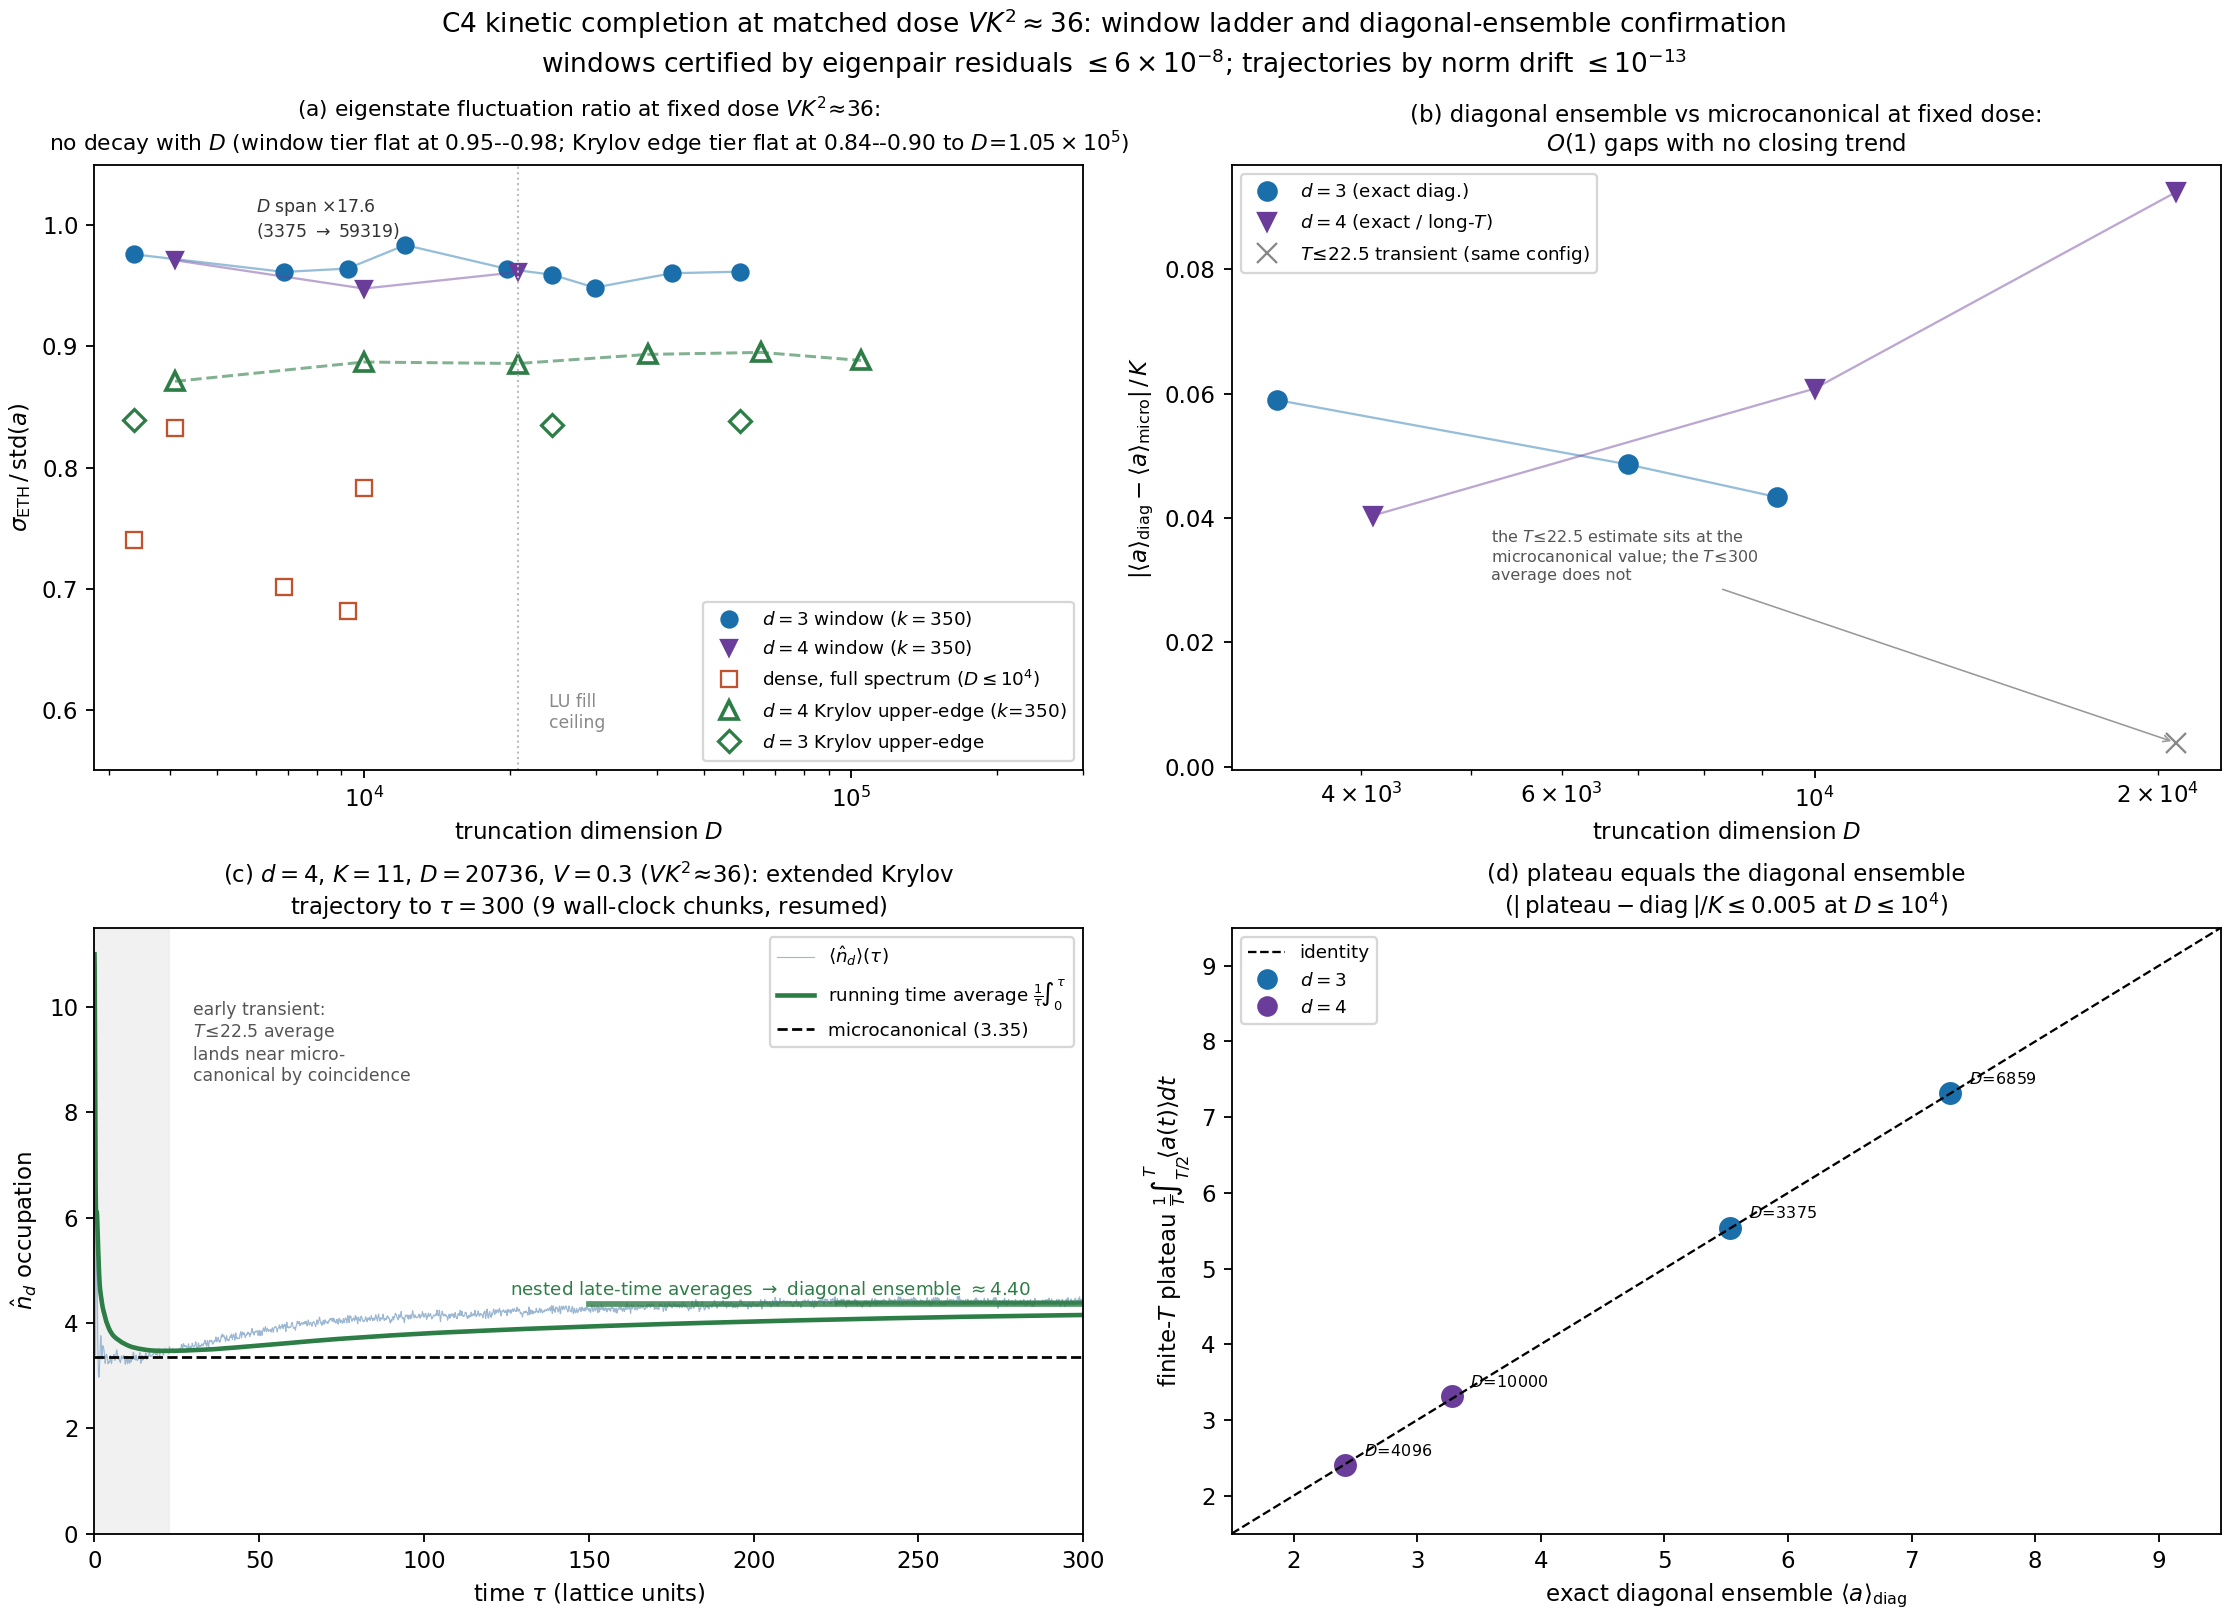
\includegraphics[width=\textwidth]{fig_c4_ladder.png}
\caption{Matched-dose ($VK^{2}\approx36$) numerics for the kinetic completion
(Remark~\ref{rem:numerics}(d)--(e)). (a)~Eigenstate fluctuation ratio
$\sigma_{\mathrm{ETH}}/\mathrm{std}(a)$ versus truncation dimension: window values
(filled) and exact full-spectrum values (open); no decay across a factor $17.6$ in $D$.
(b)~Distance of the diagonal ensemble from the microcanonical value, normalized by $K$:
$O(1)$ gaps with no closing trend; the $T\leq22.5$ estimate (cross) is a transient that
coincides with the microcanonical value. (c)~The $d=4$, $K=11$, $D=20736$, $V=0.3$
trajectory extended to $\tau=300$: observable, running time average, nested late-time
averages (diagonal-ensemble estimate $\approx4.40$), microcanonical line, and the early
transient. (d)~Finite-$T$ plateau versus exact diagonal ensemble at $D\leq10^{4}$ (identity
line).}
\label{fig:ladder}
\end{figure}

Falsifiers and test routes are listed in
Section~\ref{sec:register}.

\subsection{The Janus state}

A natural boundary condition is the vacuum: the claim that ``at the past hypothesis the
phase $1^{-i\omega_{0}\tau}=1$: time does not exist at $n=1$; time turns on when the universe
transitions to composite states.'' Under $H_{P}$ \emph{nothing} ever transitions
(Proposition~\ref{prop:frozen}), so the claim would be empty; under $H_{\mathrm{tot}}$ the vacuum
$\ket{1}$ is \emph{not} an eigenstate (because $H_{W}\ket{1}=\sum_{p}g_{p}\ket{p}$), and the
statement becomes substantive and true:

\begin{proposition}[Nucleation from the Janus state]\label{prop:nucleation}
For $H_{\mathrm{tot}}$ with $H_{W}\neq0$ and initial state $\psi(0)=\ket{1}$:
\begin{equation}
\psi(\tau)=\ket{1}-\frac{i\tau}{\hbar}\sum_{p\in P_{f}}g_{p}\ket{p}+O(\tau^{2}),
\end{equation}
so the \emph{total primon number} grows initially at rate
$d\langle\Nhat_{\mathrm{tot}}\rangle/d\tau=2\,\mathrm{Im}\,\langle\psi|H_{W}|\psi\rangle
/\hbar+O(\tau)=\frac{2\tau}{\hbar^{2}}\sum_{p}g_{p}^{2}+O(\tau^{2})>0$. The unique
zero-entropy state $\ket{1}$ is a regular point of the dynamics, not a fixed point; under
$H_{P}$ alone it is a fixed point (Proposition~\ref{prop:frozen}).
\end{proposition}

\begin{proof}
First-order time-dependent perturbation theory around the eigenstate $\ket{1}$ of $H_{P}$
(the Dyson series in $H_{W}+H_{\mathrm{hop}}$; $H_{\mathrm{hop}}$ annihilates the vacuum).
\end{proof}

Time, in this framework, is switched on by the interaction sector, with a mechanism that
exists. The stronger claims that
the actual history of the universe \emph{begins} at $\ket{1}$, and that the entropy profile is
two-sided (Janus-shaped) about that event, are boundary-condition statements and are demoted
to Conjectures $\mathsf{C7}$ and $\mathsf{C8}$; what remains as theorem is only the
uniqueness and zero entropy of the floor (Theorem~\ref{thm:spectrum} and
Section~\ref{sec:thermo}).

\section{Recurrence, Periodicity, and the Fate of Eternal Return}\label{sec:recurrence}

The anti-cyclical verdict---that prime arithmetic rigorously forbids exact cyclical
time and the universe cannot repeat---decomposes into a theorem, a correct application,
and two qualifications. This section separates them. The
resulting statement is \emph{stronger} than the slogan, because it identifies
exactly which recurrence phenomena are forbidden, which are unavoidable, and what the
boundary between them depends on.

\subsection{Linear independence of the prime logarithms}

\begin{lemma}[Fundamental-theorem independence]\label{lem:independence}
The set $\{\log p:p\in\Pr\}$ is $\Qq$-linearly independent. In particular, for distinct primes
$p,q$, the ratio $\log p/\log q$ is irrational.
\end{lemma}

\begin{proof}
Suppose $\sum_{i=1}^{r}q_{i}\log p_{i}=0$ with $q_{i}=a_{i}/b_{i}\in\Qq$ and distinct primes
$p_{i}$. Let $B=\mathrm{lcm}(b_{i})$ and $c_{i}=Bq_{i}\in\Zz$. Then
$0=\sum_{i}c_{i}\log p_{i}=\log\prod_{i}p_{i}^{c_{i}}$ (negative exponents handled by clearing
signs into the other side), so $\prod_{i}p_{i}^{c_{i}}=1$. Unique factorization forces
$c_{i}=0$ for all $i$, hence $q_{i}=0$.
\end{proof}

\subsection{Exact periodicity is forbidden}

\begin{theorem}[No exact return for generic states]\label{thm:noperiod}
Let $\psi=\sum_{n}c_{n}\ket{n}$ and let $S(\psi)=\{n:c_{n}\neq0\}$ be its support. The
following are equivalent:
\begin{enumerate}[leftmargin=1.6em]
\item There exists $\tau>0$ with $e^{-i\tau H_{P}/\hbar}\psi=\psi$;
\item There exists $T>0$ such that $\omega_{0}T\log n\in2\pi\Zz$ for every $n\in S(\psi)$;
\item The set $\{\log n:n\in S(\psi)\}$ is contained in $\alpha\,\Zz$ for some $\alpha>0$
(all supports are integer multiples of a common logarithmic unit; equivalently all $n\in
S(\psi)$ are powers of a single integer).
\end{enumerate}
In particular, if $S(\psi)$ contains any two integers $m,n$ that are not powers of a common
integer---for example any pair among $\{2,3\}$, $\{6,10\}$, $\{2,6\}$---then $\psi$ is
aperiodic: $e^{-i\tau H_{P}/\hbar}\psi\neq\psi$ for every $\tau>0$. The same holds for
$H_{\mathrm{tot}}$ whenever its spectrum is simple and contains two levels whose difference is
irrational in units of $\hbar/\omega_{0}$, which holds generically.
\end{theorem}

\begin{proof}
$e^{-i\tau H_{P}/\hbar}\psi=\sum_{n}c_{n}e^{-i\omega_{0}\tau\log n}\ket{n}$ equals $\psi$ iff
$e^{-i\omega_{0}\tau\log n}=1$ for all $n\in S(\psi)$, i.e. iff
$\omega_{0}\tau\log n\in2\pi\Zz$ for all such $n$. Setting $\alpha=2\pi/(\omega_{0}\tau)$,
this says every $\log n$ in the support lies in $\alpha\Zz$. If $m,n\in S$ and
$\log m,\log n\in\alpha\Zz$ with $\log m/\log n\notin\Qq$, the condition fails for every
$\tau$; by Lemma~\ref{lem:independence}, $\log 2/\log 3\notin\Qq$ etc.
\end{proof}

This is the rigorous core of the anti-cyclic verdict: \emph{eternal return in the exact sense
requires the support of the universal state to lie in a single geometric progression of
integers}, and no physically motivated state does.

\subsection{What is \emph{not} forbidden: three qualifications}

\begin{corollary}[Truncated systems recur]\label{cor:truncatedrecurrence}
Fix a finite truncation: primes $p\leq X$ and occupations $k_{p}\leq K$, so the Hilbert space
is finite-dimensional and the spectrum $\{E_{j}\}$ of $H_{P}$ (or of any self-adjoint
extension) is finite. Then the evolution $U(\tau)=e^{-i\tau H/\hbar}$ is a quasi-periodic
rotation, and for every state $\psi$ and every $\varepsilon>0$ the set
$\{\tau>0:\|U(\tau)\psi-\psi\|<\varepsilon\}$ is \emph{relatively dense} (there exists
$L=L(\varepsilon,\psi)$ such that every interval of length $L$ contains such a $\tau$). In
particular Poincar\'e recurrence holds in its strongest (uniform, Bohr almost-periodic) form.
This is the finite-dimensional special case of Theorem~\ref{cor:nopoincare} below, recorded
separately because it is the form in which recurrence appears in any \emph{computation}.
\end{corollary}

\begin{proof}
On a finite-dimensional space $U(\tau)=e^{-i\tau\Lambda}$ with
$\Lambda=\mathrm{diag}(E_{1},\dots,E_{d})/\hbar$; the map $\tau\mapsto
(e^{-i\tau E_{1}/\hbar},\dots,e^{-i\tau E_{d}/\hbar})$ is a continuous one-parameter
subgroup of the compact torus $\mathbb{T}^{d}$, and every orbit of a compact group rotation is
uniformly recurrent: the return times to any neighborhood of the identity are syndetic. This
is Kronecker's theorem in its group form \cite{hardywright2008}.
\end{proof}

\begin{theorem}[Uniform recurrence of the free flow, infinite system]\label{cor:nopoincare}
For \emph{every} state $\psi\in\Hil_{\mathcal{A}}$ and every $\varepsilon>0$, the set of
$\varepsilon$-return times
\begin{equation}
\Bigl\{\tau>0:\ \bigl\|e^{-i\tau H_{P}/\hbar}\psi-\psi\bigr\|<\varepsilon\Bigr\}
\end{equation}
is \emph{relatively dense} in $\Rr$. The free arithmetic flow is Bohr almost periodic for
all states, with no finite invariant measure required and no truncation assumed. What fails
is not $\varepsilon$-recurrence but its \emph{uniformity in the state}: the return-time
scale $L(\varepsilon,\psi)$ is unbounded as a function of $\psi$ (it grows with the
Diophantine complexity of the finite supports approximating $\psi$), and exact return
remains forbidden by Theorem~\ref{thm:noperiod}.
\end{theorem}

\begin{proof}
Fix $\varepsilon>0$ and $\psi=\sum_{n}c_{n}\ket{n}\in\ell^{2}$. Choose a finite support set
$F\subset\Nn_{\geq1}$ with $\sum_{n\notin F}|c_{n}|^{2}<\varepsilon^{2}/4$. The truncated
flow $\tau\mapsto\bigl(e^{-i\omega_{0}\tau\log n}\bigr)_{n\in F}$ is a continuous
one-parameter subgroup $h\colon\Rr\to\mathbb{T}^{F}$; let
$H=\overline{h(\Rr)}$, a compact connected subgroup of the torus. The $\Rr$-orbit of the
identity under left translation by $h(\tau)$ is dense in $H$ by construction, and a dense
orbit of an equicontinuous (group) action on a compact space is minimal; minimal
equicontinuous flows are uniformly recurrent, so
$T(\delta)=\{\tau:d(h(\tau),e_{H})<\delta\}$ is relatively dense for every $\delta>0$.
Taking $\delta$ small enough that all phases on $F$ deviate by less than $\varepsilon/2$
in the $\ell^{2}$ sense (finitely many constraints), we obtain
$\|U(\tau)\psi-\psi\|\leq\varepsilon/2+\varepsilon/2$ for every $\tau\in T(\delta)$, a
relatively dense set. The non-uniformity in $\psi$ follows because $F$ must grow as the
tails of $\psi$ shrink, and the Diophantine return times on $F$ are unbounded in $|F|$ (for
supports with rationally independent generators, Kronecker's theorem gives relative density
but no uniform bound: the minimal return time for $F=\{2,3,\dots,p_{|F|}\}$ grows at least
exponentially in $|F|$, since the frequencies $\log n$ are rationally independent by
Lemma~\ref{lem:independence} and simultaneous approximation of independent frequencies is
slow).
\end{proof}

The third qualification concerns the \emph{classical} multiplicative walk, and it sharpens
the boundary of the no-cycle verdict in an unexpected direction.

\begin{proposition}[P\'olya transience of the multiplicative walk]\label{prop:polya}
Consider the classical random walk on the divisibility graph of
Definition~\ref{def:multiplication} restricted to $d=|P_{f}|$ active primes: from
$k=(k_{1},\dots,k_{d})\in\Zz_{\geq0}^{d}$ step to $k+e_{j}$ with probability $1/(2d)$ and to
$k-e_{j}$ (when $k_{j}>0$) with probability $1/(2d)$, staying otherwise. Then the walk is
recurrent for $d\leq2$ and transient for $d\geq3$ \cite{polya1921}. In particular for
$d\geq3$ the walk returns to the vacuum $k=0$ (the Janus state) only finitely many times,
almost surely.
\end{proposition}

Proposition~\ref{prop:polya} has a striking interpretive reading: whether
the arithmetic universe ``cycles back to its origin'' depends on the \emph{number of active
prime modes}. With one or two primes, the multiplicative universe is recurrent---a rigorous
echo of cyclical cosmology. With three or more, it is transient, and the Janus point is a
genuinely singular origin. The absolute prohibition thus becomes a structural,
checkable dichotomy.

\subsection{The verdict on cyclical time}

Assembling the three legs: exact eternal return is impossible for states whose support spans
incommensurable integers (Theorem~\ref{thm:noperiod}); $\varepsilon$-approximate recurrence is
universal for the \emph{free} flow, at every state, with return times relatively dense but
astronomically non-uniform (Theorem~\ref{cor:nopoincare}, and
Corollary~\ref{cor:truncatedrecurrence} for the trivial finite case); and the \emph{cascading}
(or classical walk) dynamics is transient for $d\geq3$ modes (Proposition~\ref{prop:polya}),
with the interacting quantum system conjecturally non-recurrent on every physical scale
(Conjecture $\mathsf{C4}$). The philosophical consequences
are drawn in Section~\ref{sec:philosophy}; the essential point is that the framework's
anti-cyclical verdict survives as a \emph{layered} statement---exact return forbidden as a
genuine theorem, practical return driven out of reach by Diophantine slowness, transience
of the cascade for three or more active modes---rather than as an absolute metaphysical
prohibition. The free arithmetic sector, left to itself, is the \emph{most} recurrent object
in the theory (Bohr almost periodicity for all states, Theorem~\ref{cor:nopoincare}); all
irreversibility is therefore manufactured by the interaction sector and the boundary
condition, never by the spectrum. This is the sharpest available form of the intuition
that ``the river never circles back,'' and it is also the form most useful to
the arrow-of-time analysis of Sections~\ref{sec:time} and~\ref{sec:philosophy}.
